\documentclass{article}\usepackage[]{graphicx}\usepackage[]{color}

\title{Needs a title}
\author{Sang Woo Park, Benjamin M Bolker}

\usepackage{tabularx}

\usepackage{amsmath}
\usepackage{natbib}
\usepackage{hyperref}
\bibliographystyle{chicago}
\date{\today}

\newcommand{\etal}{\textit{et al.}}

\newcommand{\fref}[1]{Fig.~\ref{fig:#1}}
\IfFileExists{upquote.sty}{\usepackage{upquote}}{}
\begin{document}

\maketitle

\section{Introduction}

The evolution of sexual reproduction still remains to be explained \citep{otto2009evolutionary}.
Despite being the dominant mode of reproduction \citep{vrijenhoek1998animal}, sexual reproduction is followed by many costs \citep{lehtonen2012many}.
Perhaps the most often mentioned is the cost of producing males \citep{smith1978evolution}.
As males cannot produce offspring, a sexually reproducing population is expected to be outgrown by an asexually reproducing counterpart that can grow twice as fast (given that the sexual population produces 50\% males and 50\% females).
The infamous \emph{two-fold cost of sex} \citep{smith1978evolution} relies on the assumption that everything else is equal but this is not necessarily true.
So what drives sex to persist?

One explanation for sex is the Red Queen Hypothesis \citep{bell1982masterpiece}.
The Red Queen Hypothesis predicts sexually reproducing hosts to overcome the cost of sex under strong parasite selection by producing genetically diverse offspring that are resistant to infection \citep{jbs1949disease, jaenike1978hypothesis, hamilton1980sex}.
Host parasite coevolution constantly creates selective advantage for rare genotypes (hence osccilation in genotypic frequencies) and allows for sexual reproduction to persist in the host population \citep{clarke1976ecological, hamilton1980sex}.

Since the conception of the Red Queen Hypothesis, much of the theoretical work has focused on figuring out conditions under which parasite selection can maintain sexual reproduction in the host population.
\cite{may1983epidemiology} first noted that parasites must be extremely virulent to maintain sexual reproduction.
Later models showed that virulence is an important factor but it is possible for sexual and asexual hosts to coexist at intermediate virulence \citep{howard1994parasitism}.
\cite{agrawal2002infection} compared wide range of infection genetics that determine parasite resistance and the dynamics that arise from different genetic architecture.
Some studies took a departure from a typical population genetics framework and showed that incorporating ecological and epidemiological details to the model can support sexual reproduction in the host population \citep{galvani2001antigenic, galvani2003maintenance, lively2009maintenance, lively2010epidemiological}.
Recent studies showed that host genetic diversity plays an important role in determining the selection for sex [CITE].

On the other hand, empiricists have mostly focused on indirect tests that stem from the hypothesis.
Popular among them are local adaptation, time-lagged selection, and association between parsites and host reproductive mode (see \cite{tobler2008expanding} and \cite{vergara2014infection} for reviews).
Recent works on experimental systems have provided more direct support for the hypothesis \citep{auld2016sex, slowinski2016coevolutionary}.
A notable example is a snail population in New Zealand that serve as an intermediate hosts for trematodes [CITE].
Through several decades of work, Lively [CITE] demonstrated that the population appears to satisfy essential requirements and provide support for the hypothesis.

While the Red Queen Hypothesis has gained reasponably support both theoretically and empirically, there still remains a gap between theory and data.
Many models for Red Queen Hypothesis rely on simplifying assumption that are not applicable to natural populations and make predictions based on assumed parameters.
In particular, none of the Red Queen models reviewed by \cite{ashby2015diversity} use statistical tools to relate the model to data.
However, there are exceptions:
\cite{lively1992parthenogenesis} initially postulated that infection prevalence should be positively correlated with frequency of sexual hosts. 
\citep{lively2001trematode} then formalized the idea with a mathematical model and confirmed his prediction with a snail-trematode system.
Many other emprical works have successfully demonstrated the positive correlation \citep{lively2002temporal, kumpulainen2004parasites, vergara2013geographic, mckone2016fine} but surprisingly such correlation was not observed in a different snail-trematode system \citep{dagan2013clonal}.

Here, we try to bridge the gap further.
We extend the model used by \cite{lively2010epidemiological} to include stochasticity and population structure and fit it the to data from \cite{dagan2013clonal, mckone2016fine, vergara2014infection} using Approximate Bayesian Computation (ABC).
Using posterior distributions obtained from the fits, we perform power analysis to test the prediction that infection prevalence is positively correlated with frequency of sexual reproduction \cite{lively2001trematode}.

\section{Methods}

\subsection{Study systems}

We consider two snail-trematode populations in New Zealand \citep{vergara2014infection, mckone2016fine} and a similar snail-trematode population in Isral \citep{dagan2013clonal}. 
The snail-trematode system has been extensively studied under the context of the Red Queen Hypothesis [CITE] so we expect a simple Red Queen model to fit well.
Data collected by \cite{dagan2013clonal} and \cite{vergara2014infection} were obtained from their Dryad repositories \citep{dryad_f5t56, dryad_29nk3_2} and data by \cite{mckone2016fine} was extracted from their figure.

\subsection{Model}

We model obligate sexual hosts competing with obligate asexual hosts in multiple population by extending the model introduced by \cite{lively2010epidemiological}.
A model that \cite{lively2010epidemiological} used is essentially an SI model on a discrete time scale with natural mortality and virulence (reduced offspring production by infected hosts).
It is a suitable canditate for this study as it captures essential structures that are present in basic epidemiological and population biology models and is general enough to be applied to broad range of natural systems.
We do not consider mechanistic details of the snail-trematode system such as life history of trematodes \citep{vergara2014infection}.
We incorporate population structure and allow for mixing between populations.
Each population can be considered as a sampling site in the observed populations.

All hosts are assumed to be diploids with two biallelic loci, and parasites are assumed to be haploids.
Let $S_{ij}^k(t)$ and $A_{ij}^k(t)$ be the number of sexual and asexual hosts with genotype $ij$ from population $k$ at generation $t$. 
For simplicity, we drop the superscript representing population and write $S_{ij}(t)$ and $A_{ij}(t)$;
every population is modeled using the same equations unless noted otherwise.
Following \cite{lively2010epidemiological}, the expected number of offsprings (without recombination or outcrossing) produced by a sexual population is given by
\begin{equation}
S_{ij}' = c_b (1-s) \left(W_U S_{ij,U} (t) + W_I S_{ij,I} (t)\right),
\end{equation}
where $s$ is the proportion of males produced by sexual hosts, $S_{ij, U}$ and $S_{ij,I}$ are the number of uninfected and infected sexual hosts in a population.
$W_U$ and $W_I$ represent their corresponding fitnesses.
We allow for cost of sex to vary by multiplying a scale parameter, $c_b$, to the growth term ($2/c_b$ corresponds to two fold cost of sex) \citep{ashby2015diversity}.
Equivalently, $S_{ij}'$ is the amount of genotypic contribution by sexual hosts to the next generation.

Asexual hosts are assumed to be strictly clonal. Then, the expected number of offsprings produced by an asexual population is given by
\begin{equation}
A_{ij}' = W_U A_{ij,U} (t) + W_I A_{ij,I} (t),
\end{equation}
where $A_{ij, U}$ and $A_{ij,I}$ are the number of uninfected and infected asexual hosts in a population.

We assume mixing between populations occur at rate $\epsilon_{\textrm{mix}}$.
Then, the expected number of offspring in the next generation (accounting for contributions from all populations) is given by
\begin{equation}
\begin{aligned}
\mathrm{E}\left(S_{ij}^k(t+1)\right) &= f_{\textrm{sex}}\left((1 - \epsilon_{\textrm{mix}}) \left(S_{ij}^k\right)' + \frac{\epsilon_{\textrm{mix}}}{n_{\textrm{population}}-1} \sum_{h \neq k} \left(S_{ij}^h\right)'\right),\\
\mathrm{E}\left(A_{ij}^k(t+1)\right) &= (1 - \epsilon_{\textrm{mix}}) \left(A_{ij}^k\right)' + \frac{\epsilon_{\textrm{mix}}}{n_{\textrm{population}}-1} \sum_{h \neq k} \left(A_{ij}^h\right)',\\
\end{aligned}
\end{equation}
where $f_{\textrm{sex}}(x)$ is the function that models sexual reproduction, including recombination at a rate $r_{\textrm{host}}$ and outcrossing, and $n_{\textrm{population}}$ is the number of populations modeled.
We then take a poisson random variable to simulate process error and allow for stochastic migration to avoid fixation:
\begin{equation}
\begin{aligned}
S_{ij}^k(t+1) &\sim \mathrm{Poisson}\left(\lambda=\mathrm{E}\left(S_{ij}^k(t+1)\right)\right) + \mathrm{Bernoulli}\left(p=p_{ij,\textrm{sex}}\right),\\
A_{ij}^k(t+1) &\sim \mathrm{Poisson}\left(\lambda=\mathrm{E}\left(A_{ij}^k(t+1)\right)\right) + \mathrm{Bernoulli}\left(p=p_{ij, \textrm{asex}}\right),
\end{aligned}
\end{equation}
where $p_{ij,\textrm{sex}}$ and $p_{ij, \textrm{asex}}$ are the probability of a sexual and an asexual host with genotype $ij$ entering the popualation.

Infection is modeled using the matching alleles model \citep{otto1998evolution}.
We assume that heterozygous individuals are equally susceptible to parasites that match either haplotypes.
The expected number of infected hosts that carry parasite with genotype $i$ at generation $t$ is given by:
\begin{equation}
I_{i}(t) = \sum_{p} 2^{\delta_{ij}} \left( S_{ip,i,I}(t) + A_{ip,i,I}(t)\right),
\end{equation}
where $\delta_{ij}$ is kronecker delta.
$S_{ip,i,I}$ and $A_{ip,i,I}$ represent the expected numbers of sexual and asexual hosts infected with genotype $i$ parasite. 
Following \cite{ashby2015diversity}, we assume that mutation can occur in one locus with probability $r_{\textrm{parasite}}$. 
We also allow for external migration of an infected host carrying parasite $i$ with probability $p_{i, \textrm{parasite}}$ to avoid fixation.

The amount of infectious contacts made by infected hosts from a population is given by $\lambda_i^k = \beta^k {I_i'}^k(t)$, where $\beta^K$ is the transmission rate at each population, and $I_i'(t)$ is the number of infected hosts accounting for mutation and migration.  
Since we allow for mixing between population, infected hosts in a population can make contact to susceptible hosts in other populations as well.
Then, all infectious contacts made by infected hosts that applies to a host in a single population is
\begin{equation}
\lambda_{i, \textrm{total}} = (1 - \epsilon_{\textrm{site}}) \lambda_i + \frac{\epsilon_{\textrm{site}}}{n_\textrm{site}-1} \sum_{l \neq k} \lambda_i^l
\end{equation}
Then, the force of infection that a susceptible host experiences is given by
\begin{equation}
\mathrm{FOI}_{ij}^k = \frac{\lambda_{i, \textrm{total}}  + \lambda_{j, \textrm{total}}  }{2 N(t+1)}
\end{equation}
The probability of infection for a host with genotype $ij$ at site $k$ in the next generation is
\begin{equation}
P_{ij}^k(t+1) = 1 - \exp\left(\mathrm{FOI}_{ij}^k\right).
\end{equation}

Finally, number of infected hosts in the next generation is determined by a binomial process:
\begin{equation}
\begin{aligned}
S_{ij,I} (t+1) &\sim \mathrm{Binom}(S_{ij} (t+1), P_{ij}),\\
A_{ij,I} (t+1) &\sim \mathrm{Binom}(A_{ij} (t+1), P_{ij}).
\end{aligned}
\end{equation}
Expected number of individuals infected by parasites with genotype $i$ in the next generation is given by a ratio of $\lambda$:
\begin{equation}
\begin{aligned}
S_{ij,i,I}(t+1) &= \frac{\lambda_{i, \textrm{total}}}{\lambda_{i, \textrm{total}} + \lambda_{j, \textrm{total}}} S_{ij,I}(t+1)\\
A_{ij,i,I}(t+1) &= \frac{\lambda_{i, \textrm{total}}}{\lambda_{i, \textrm{total}} + \lambda_{j, \textrm{total}}} A_{ij,I}(t+1)
\end{aligned}
\end{equation}

\subsection{Simulation design and parameterization}

Most Red Queen models have studied a competition between a single asexual genotype and sexual genotypes or have assumed equal genetic diversity of asexual and sexual hosts \citep{ashby2015diversity} but neither of these assumptions are realistic.
Instead, \cite{ashby2015diversity} adopted a more realistic approach by allowing for stochastic migration of an asexual genotype to a population.
Here, we combine these methods.
We allow for stochastic migration of asexual hosts with different genotypes but fix number of asexual genotypes (denoted by $G_{\textrm{asex}}$) that can be present in the system, 
while the number of sexual genotypes ($G_{\textrm{sex}}$) that can be present in the population remains equal to the size of the genotypic space ($=10$ in diploid hosts with two biallelic loci).

In the beginning of every simlation, $G_{\textrm{asex}}$ is randomly chosen between 1 and 10 and asexual genotypes that can be introduced to the population are uniformly sampled from the entire genotypic space.
To account for differing number of sexual and asexual genotypes, we let 
\begin{equation}
\begin{aligned}
p_{ij, \textrm{sex}} &= 1-(1-p_{\textrm{host}})^{1/G_\textrm{sex}},\\
p_{ij, \textrm{asex}} &=
\begin{cases}
1-(1-p_{\textrm{host}})^{1/G_\textrm{asex}} & \text{if } ij \in \{\text{asexual genotypes}\} \\
0 & \text{otherwise}
\end{cases},
\end{aligned}
\end{equation}
where $p_{\textrm{host}}$ is the probability that at least one sexual and asexual host enters the population in a generation. We scale the probability of infected host carrying parsite genotype $i$ in a similar way for interpretability:
\begin{equation}
p_{i, \textrm{parasite}} = 1 - (1-p_{\textrm{infected}})^{1/4},
\end{equation}
where $p_{\textrm{infected}}$ is the probability that at least one infected host enters the population in a generation.

Each simulation consists of 40 populations. Every population consists of 2000 sexual hosts where 80 of them are infected. They are assumed to be in Hardy-Weinberg equilibrium with ratio between alleles being exactly half. Transmission rate parameter, $\beta$, is randomly drawn from a lognormal distribution with parameters $\beta_{\textrm{meanlog}}$ and $\beta_{\textrm{sdlog}}$ for each population. Simulation runs for 500 generations without introduction of asexuals. At generation 501, 10 asexual hosts of a single genotype are introduced to each population (note that asexual genotype introduced can vary across population) and simulation runs for 600 generations while allowing for stochastic migration of asexuals as well.

\subsection{Approximate Bayesian Computation}

We use Approximate Bayesian Computation (ABC) to fit the model \citep{toni2009approximate}.
ABC relies on comparing summary statistics of observed data and those of simulated data and can be particularly useful when the exact likelihood function is not available [CITE?].
We consider mean proportion of infected and sexually reproducing snails in the system and variation in these proportions -- measured by coefficient of variation (CV) -- across space and time as summary statistics of interest.

For each sample from the posterior, the model is simulated and a subsample from the simulated data is drawn so that the number of simulated population is equal to the number of sites collected in a study.
Then, the summary statistics are calculated by considering last 100 generations of simulated data and the parameter sample as well as the simulation generated by the sample is accepted if the distance between simulated and observed data (measureed by the absolute sum of differences in summary statistics) is less than the tolerance value.
By simulating greater number of populations than number of sampled sites, we account for uncertainty in unobserved population as well as interaction between populations.

We use uninformative priors for all parameters except $c_b$, a scale parameter for the cost of sex.
The prior distribution for the scale parameter is chosen so that 95\% quantile of cost of sex (2/$c_b$) is approximately equal to the 95\% confidence interval reported by \cite{gibson2017two} (see ??? for the list of parameters).
As \cite{dagan2013clonal} and \cite{mckone2016fine} report proportion of males, instead of proportion of sexual hosts, we double the proportion of males reported when we fit the model.

To allow for more efficient estimation of the posterior distribution, we use Sequential Monte Carlo \cite{turner2012tutorial} (see Appendix for details).

\subsection{Power analysis}

To calculate the power to detect positive correlation between infection prevalence and frequency of sexual hosts, we simulate an observed sample by drawing a random multinomial sample from simulated data.
For simplicity, we assume that a year contains of two snail generations [CITE] and that samples are taken within a short period of time.
For each simulation from the posterior distributions, we start by setting a reference generation to generatation 1001 and choosing $n$ populations at random from 40 simulated popoulations.
For each selected population, hosts are divided into four categories based on their infection status (infected/uninfected) and reproductive mode (asexual/sexual),
and mean proportion of hosts in each category is calculated by averaging over two consecutive generations.
A multinomial sample of size $m$ is drawn from each selected population independently based on the four categories. 
Positive correlation between proportion of infected hosts and proportion of sexual hosts is tested using Spearman's rank correlation at 5\% significance level.
We repeat the process 100 times for each simulation from a posterior distribution.

\section{Results}

Our simple Red Queen model with population structure can reproduce infection prevalence and frequency of sexual hosts observed acrosss three different snail-trematode systems reasonably well.
A notable difference is that our model tends to overestimate mean infection prevalence across all three systems (\fref{smcsumm}).
In particular, \cite{mckone2016fine} reported mean infection prevalence of 5.1\% but the mean (95\% quantile) estimate of the fitted model is 23.7\% (9.1\% - 40.3\%).
The model fitted model \cite{vergara2014infection} population underestimates mean frequency of sexual hosts in by almost 10\% when compared with the mean estimate but the observed mean frequency still lies within a reasonable range of fitted values.
Even though model fitting was performed by minimizing the absolute distance between observed and simulated summary statistics, there is large variation in fitted summary statistics because we take uncertainty in unobserved populations into account.

\begin{figure}[!ht]
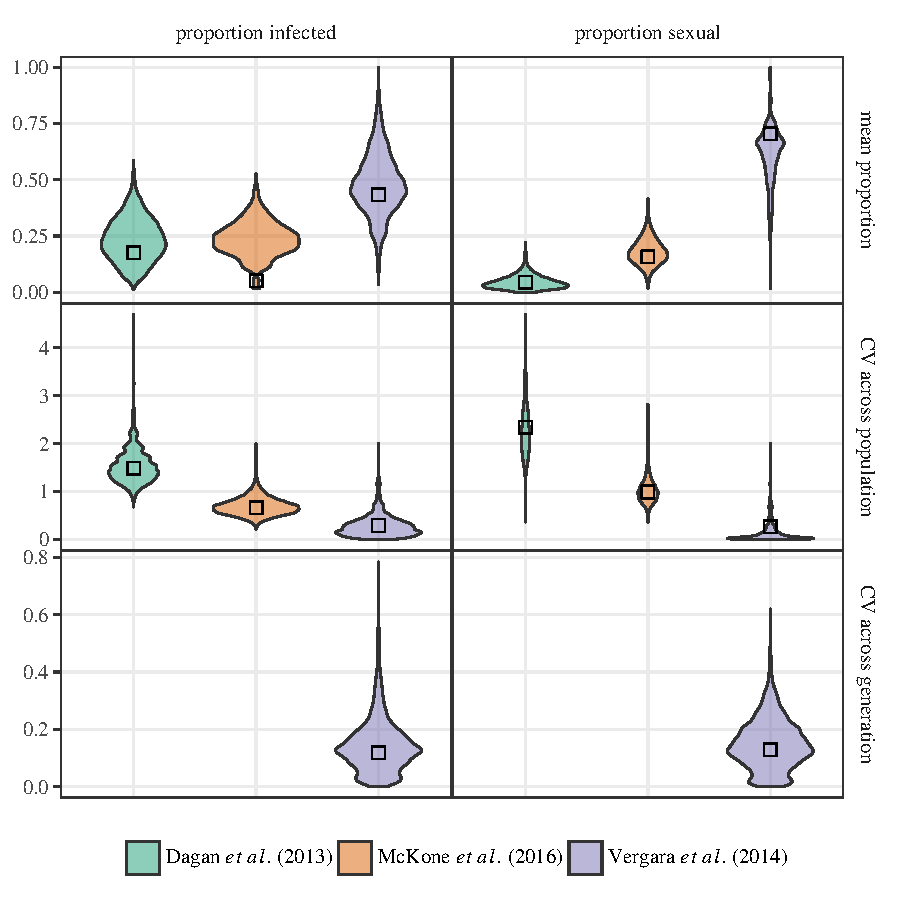
\includegraphics[width=\textwidth]{../fig/smc_summary.pdf}
\caption{{\bf Summary statistics of the observed data v.s. summary statistics of the simulated data from the posterior samples.}
Violin plots show distribution of summary statistics from each simulated set. For each simulated data set accepted along with a posterior parameter sample, simulated populations are sampled at random 100 times so that each sample consists of equal number of populations as number of sites in fitted data. Then, summary statistics are calculated for each sample by taking last 100 generations. Squares represnt observed summary statistics.
}
\label{fig:smcsumm}
\end{figure}

To further diagnose the fit, we compare the relationships between infection prevalence and frequency of sexual hosts predicted by the model with those observed across three systems (\fref{ivs}).
Despite being able to reproduce summary statistics reported by \cite{dagan2013clonal} well, 
our model is unable to predict qualitative trend bewteen proportion of sexual hosts and proportion of infected hosts (\fref{ivs}; \cite{dagan2013clonal}).
While both simulated data and observed data mostly consist of asexual populations,
our model predicts some amount of sexual reproduction to be maintained when infection prevalence is greather than 20\%. 
On the other hand, the data provided by \cite{dagan2013clonal} shows that sexual reproduction is only maintained at low levels of infection prevalence and is barely maintained otherwise.
Similarly, overestimation of infection prevalence is more strongly pronounced in \fref{ivs}.
We find that our model is not able to support high level of sexual reproduction at a low prevalence.
Due to such badness of fit, we exclude fits to \cite{dagan2013clonal} and \cite{mckone2016fine} from discussing parameter estimates and power analysis.

\begin{figure}[!ht]
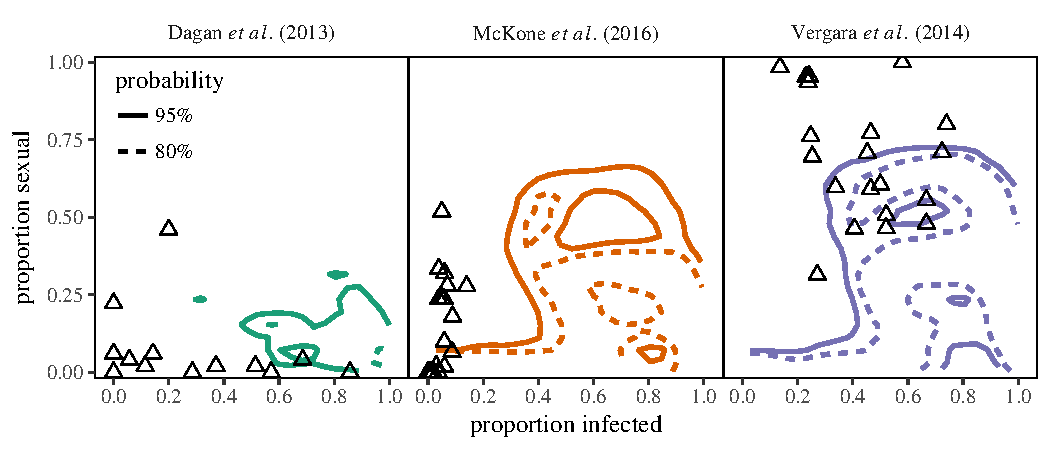
\includegraphics[width=\textwidth]{../fig/simulated_data.pdf}
\caption{{\bf Comparison in trends of the observed data v.s. simulated data from the posterior samples.}
Solid circles represent a population within a simulation. Triangles represent observed data.}
\label{fig:ivs}
\end{figure}

The most striking result from \fref{ivs} is that there is a region (around 10\%-60\% prevalence) in which proportion of infected hosts decreases while proportion of sexual hosts increases (most clearly seen from the fits to \cite{mckone2016fine} and \cite{vergara2014infection}).
As transmission rate ($\beta$) increases, selection for sexual hosts increases but increasing number of resistant offsprings prevents further infection from occuring. 
Depending on the strength of infection and amount of resistant offsprings produced, infection prevalence may decrease of stay constant.
This region connects the overlap in prevalence between sexual and asexual populations noted by \cite{lively2001trematode}
We find that proportion of sexual hosts decreases when infection prevalence is very high.
Decrease in fitness of sexual hosts with increase in prevalence was predicted by \cite{ashby2015diversity} but is also observed in an earlier work by \cite{lively2010epidemiological} (not discussed in the paper).

Parameter estimates for \cite{vergara2014infection} are presented in \fref{smcparam}.
The most surprising result is that the posterior distributions of the scale parameter for cost of sex, $c_b$, is much wider than the prior distribution and have noticeably higher mean: (mean (95\% credible interval)) 1.29 (0.79-2.01).
\cite{ashby2015diversity} defined $c_b$ as additional costs and benefits of sex, where $c_b=1$ corresponds the two fold cost.
Under their interpretation, our estimate corresponds to the following mean and 95\% CIs for cost of sex: 1.55 (1.00-2.52).
Note that some posterior samples range $c_b > 2$, corresponding to faster growth rate of sexual hosts than asexual hosts.
Simulated data from these posterior samples mostly consist of populations with almost 100\% sexual hosts.
While these estimates are not entirely impossible given that \cite{vergara2014infection} observed almost 100\% sexual snails in one of their sampling sites throughout 5 years, their observation is likely to be a sampling artifact since an earlier work sampled at the same site reported much lower frequency of sexual snails \citep{vergara2013geographic}. %% TODO: double check sources

\begin{figure}[!ht]
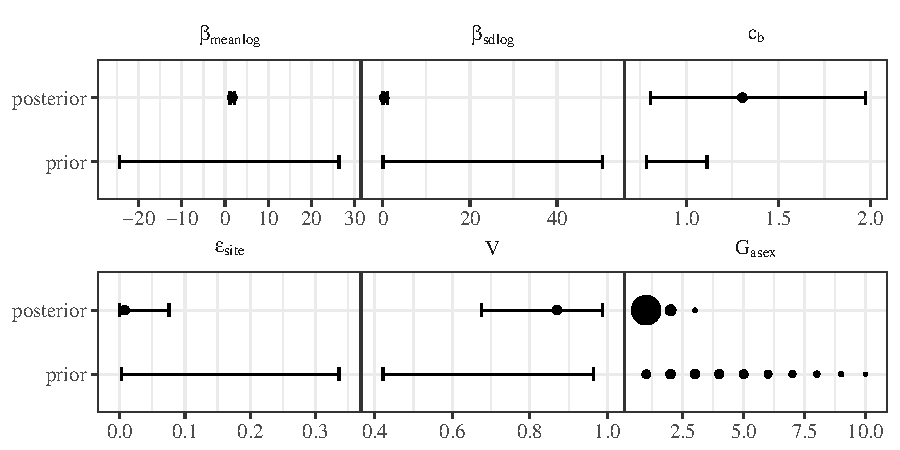
\includegraphics[width=\textwidth]{../fig/verg_post.pdf}
\caption{{\bf Parameter estimates from Sequential Monte Carlo Approximate Bayesian Computation.}
Lines repreesnt 95\% quantile and points represent mean posterior estimates. 100 posterior samples were obtained from SMC ABC. Prior distributions are specified in [TODO].
}
\label{fig:smcparam}
\end{figure}

The model estimates high virulence overall: (mean (95\% CI)) 88.8\% (75.0\%-99.2\%).
In contrast to \cite{lively2010epidemiological}, who modeled 1 asexual genotype competing with 9 sexual genotypes, our model estimate shows that higher asexual to sexual genotypic ratio can be supported ($G_{\textrm{asex}}$ panel in \fref{ivs}).
90 out of 100 posterior samples estimate $G_{\textrm{asex}} = 1$; 9 samples estimate $G_{\textrm{asex}} = 2$; and 1 sample estimates $G_{\textrm{asex}} = 3$.
However, we find that it is still necessary for sexual hosts to have higher genetic diversity than asexual hosts.

Finally, a power analysis show that the power for detecting a positive correlation between infection prevalence and frequency of sexual hosts in \cite{vergara2014infection} population is almost 0 (\fref{power}).
We find that there is much higher (but still low) power to detect a negative correlation.
Increasing number of samples per site has small effect on power once the sample size greater than 50.
Increasing number of sites leads to greater increase in power but the power appears to saturate as number of sites increases.

\begin{figure}[!ht]
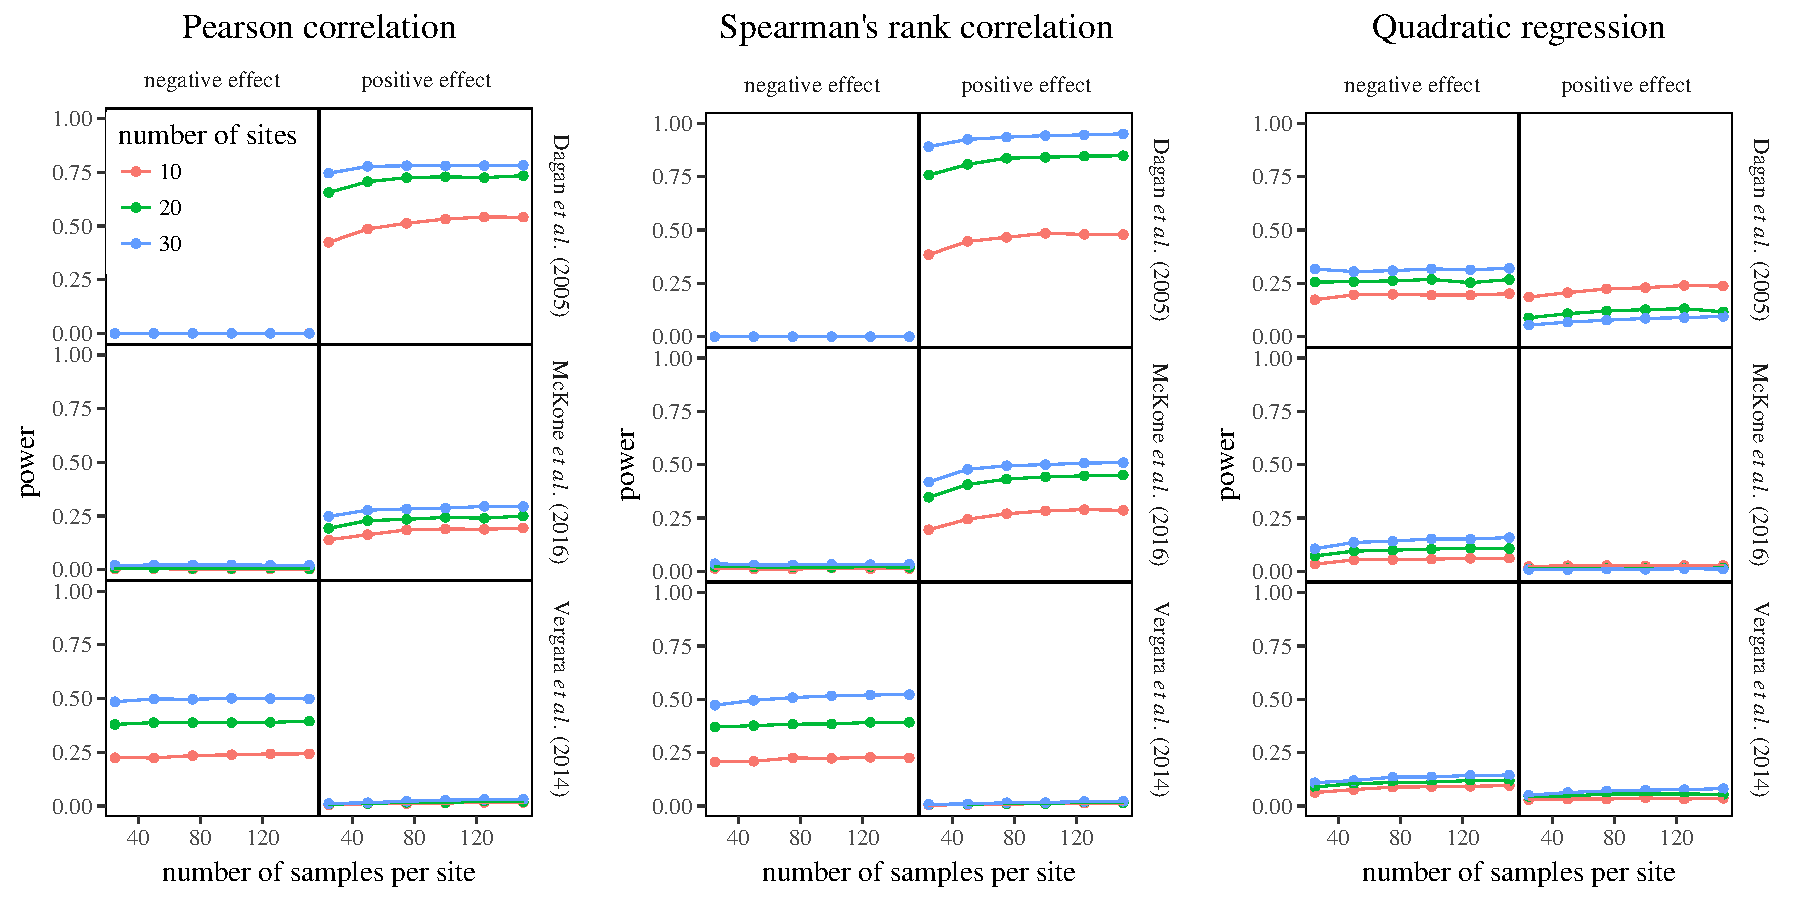
\includegraphics[width=\textwidth]{../fig/power.pdf}
\caption{{\bf Power to detect a statistically clear correlation between infection prevalence and frequency of sexual hosts.}
(a) Power to detect a positive correlation. 
(b) Power to detect a negative correlation. 
(c) (Contour) power to detect a positive correlation as a function of transmission rate parameters and (points) marginal posterior distributions.
Spearman's rank correlation was used to test for correlation between infection prevalence and frequency of sexual hosts in simulated data from the posterior distributions.
Contour plot is created by taking the mean posterior estimates and assuming 20 sites and 100 samples per site.
}
\label{fig:power}
\end{figure}

\section{Discussion}

Our results challenge ways in which the Red Queen Hypothesis for sex has been studied.
Previous modeling studies have either relied on assumed parameters [CITE] or explored parameter spaces [CITE]
to understand sexual reproduction maintained by host parasite coevolution.
Here, we show that (1) model parameters are estimable and (2) a simple Red Queen model with population structure can reproduce key summary statistics observed across three different snail systems (\fref{smcsumm}).
While our model is able to reprouce observed summary statistics, there still remain some discrepancies between model prediction and observed relationship between infection prevalence and frequency of sexual hosts across populations.
These discrepancies suggest a simple host-parasite model is not sufficient to explain sexual reproduction observed in nature.
% We also find that detecting a positive correlation between infection prevalence and frequency of sexual hosts is difficult (\fref{power}) and hence not a good measure for measuring the effects of the Red Queen.

A model that does not fit well can sometimes tell us more about the system of interest than a model that fits well.
For example, there is a clear mismatch between the model and the data presented by \cite{dagan2013clonal} (\fref{ivs}).
The snail populations studied by \cite{dagan2013clonal} live in intrinsically different environments from two other snail populations that we consider.
For example, some habitats are subject to seasonal flash floods, which can affect reproductive strategies of snails \citep{ben2007temporal}.
Althuogh we cannot estimate the strength of the effect of environment on sexual reproduction of snails relative to that of the effect of parasites, it is likely to be a cause of the bad fit.
We conclude that the Red Queen Hypothesis alone cannot explain maintenance of sexual reproduction in this population.

The only system that our model could resemble fairly well is one studied by \cite{vergara2014infection}.
In order for our model to produce similar summary statistics as those observed in nature, it requires the scale parameter ($c_b$) for the cost of sex to have mean greater than 1 (\fref{smcparam}).
A model that assumes two fold cost of sex ($c_b=1$) would not have fitted well.
However, from an inferential point of view, $c_b > 1$ does not necessarily imply that cost of sex is less than two fold.
We interpret an estimate of $c_b > 1$ as amount of compensation required in order for the model to reproduce observed data.
Additional compensation can include less than two fold cost of sex or any other mechanisms that can promote sex.

A suitable candidate for model compensation is increase in host genetic diversity.
Although exact genetic architecture that determines trematode infecion in snails (e.g., loci involved in parasite resistance) is not known {CITE}, genetic diversity of snails that have been documented is far greater than what we have assumed \citep{king2011parasites, dagan2013clonal}.
In addition, increasing genetic diversity of the model may resolve overestimation of infection prevalence (\fref{smcsumm}).
Previous studies have shown that moderately high genetic diversity can allow sexual hosts to escape infection more easily and therefore reduce prevalence of infection given similar amount of sexual reproduction \citep{lively2010effect, king2012does, ashby2015diversity}.
Overall, our results indicate that more modeling effort is required to understand prevalence of sexual reproduction in nature.

Our power analysis (\fref{power}) constrasts with the positive correlation predicted by \cite{lively1992parthenogenesis, lively2001trematode} and findings of many empirical studies that have confirmed the prediction \citep{lively1987evidence, lively2002temporal, kumpulainen2004parasites, vergara2013geographic, mckone2016fine}.
The power analysis predicts almost no power for detecting a positive corrleation in the population studied by \cite{vergara2014infection} and relatively higher but still low power for detecting a negative correlation.
This result may appear to contradict an earlier work by \cite{vergara2013geographic} that reported a positive correlation between between infection prevalence and male frequency in the same lake but there is a simple explanation for the difference.
The key premise behind the postive correlation predicted by \cite{lively2001trematode} is that there must be large variation in infection prevalence.
In particular, range of prevalnece must be wide enough so that the sample includes sites with almost no infected hosts (hence no sexual hosts) and those with reasonably high proportion of infected hosts to maintain sexual reproduction through parasitism \citep{lively2001trematode}.
Since all four habitats studied by \cite{vergara2014infection} consists of populations with high prevalence and high frequency of sexually reproducing hosts, positive correlation vanishes.
Instead, studying a system with larger variation and lower mean prevalence would yield much high power (\fref{power}(c)).

% While predicting a positive correlation between prevalence of infection and frequency of sexual hosts, \cite{lively2001trematode} also noted that there is a region at which expected infection prevalence overlaps between sexual and asexual populations. 
% Within this region lies the association between increase in sexual reproduction and decrease in infection prevalence observed in \fref{ivs}.
On the other hand, negative correlation between prevalence of infection and frequency of sexual hosts can be explained by cycling of host and parasite populations.
A main component of the Red Queen Hypothesis is that negative frequency dependence drives oscillation in both host and parasite population \citep{hamilton1980sex}.
When temporal variation is taken into account, association between infection prevalence and frequency of sexual hosts can change depending on what phase each of the sample population is going through in its cycle (\fref{cycle}).
The negative correlation in the population does not contradict the positive correlation predicted by \cite{lively2001trematode} because their prediction did not take temporal variation into account.

\begin{figure}[!ht]
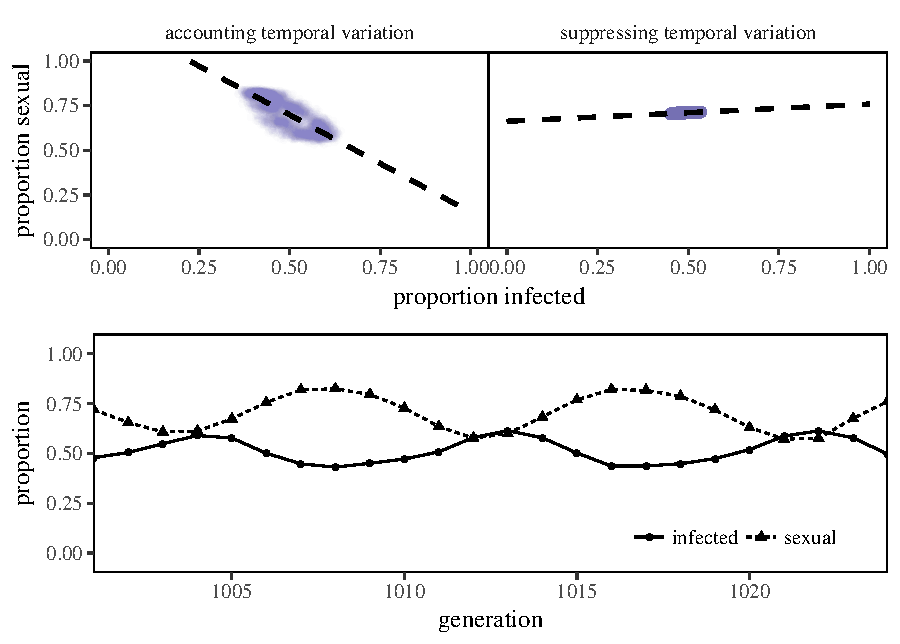
\includegraphics[width=\textwidth]{../fig/cycle_example.pdf}
\caption{{\bf Simulated data from the posterior distribution fitted to \cite{vergara2014infection}.}
A particular simulation is chosen from the posterior distributions to demonstrate that it is possible to predict opposite relationship when temporal variation is taken into account. (Top left) each point represents proportion of infected hosts and proportion of sexually reproducing hosts of each population at each generation. Last hundred generations are plotted. (Top right) each point represents mean proporiton of infected hosts and mean proportion of sexually reproducing hosts of each population averaged over the last hundred generations. Dashed lines represent least squares fit to all point. (Bottom) A typical host parasite cycle observed in a population from this simulated data. %% TODO: need to report parameter values?
}
\label{fig:cycle}
\end{figure}

%% still thinking about conclusion

\bibliography{redqueen}
\end{document}
